\documentclass[12pt,a4paper,dvipdfmx,titlepage]{jsarticle}

\usepackage[top=25truemm,bottom=25truemm,left=25truemm,right=25truemm]{geometry}

\usepackage{graphicx}

\usepackage{url}
\bibliographystyle{jplain}

\usepackage{listings}
\usepackage{xcolor}

\definecolor{codegreen}{rgb}{0,0.6,0}
\definecolor{codegray}{rgb}{0.5,0.5,0.5}
\definecolor{codeorange}{rgb}{0.8,0.4,0}
\definecolor{backcolour}{rgb}{1,1,1}

\lstdefinestyle{mystyle}{
    backgroundcolor=\color{backcolour},
    commentstyle=\color{codegreen},
    keywordstyle=\color{magenta},
    numberstyle=\tiny\color{codegray},
    stringstyle=\color{codeorange},
    basicstyle=\ttfamily\footnotesize,
    breakatwhitespace=false,
    breaklines=true,
    captionpos=b,
    keepspaces=true,
    numbers=left,
    numbersep=8pt,
    showspaces=false,
    showstringspaces=false,
    showtabs=false,
    tabsize=2
}

\lstset{style=mystyle}

\begin{document}

\title{
    データサイエンス演習 最終レポート\\
    \large 気象情報と旅客用航空機遅延時間の分析
}

\author{
	\gt{9 うに}\\
	\gt{1021120 及川 寛太}
}

\date{2023年8月3日}

\maketitle

\section*{概要}
本レポートでは、気象情報と旅客用後期遅延時間との関連を、気象庁と日本航空 (以下、JAL) が公開しているデータを用いて分析した。いくつかの空港をピックアップし、それぞれの空港を発着し、遅延が発生した便のデータをデータベースに収集した。また、その期間の気象データを収集した。それぞれのデータをさまざまな条件をもとに結び付け、重回帰分析をして、どの気象要因が遅延時間に最も影響を与えているのかを明らかにしようとした。モデルの評価の結果、スコアが低く結果の信憑性は乏しいが、分析の過程で改善すべき点をいくつか考察した。また、本レポートの最後に、実装したプログラムのソースコードを掲載した。

\section*{背景・目的}
旅客用航空機が遅延・欠航する理由はいくつかある。国土交通省\cite{delayAndCancellationRate}によると、令和5年1月から3月の間、JALの遅延理由として、機材繰りが最も多く、天候が次に多かった。欠航理由としては、天候が最も多かった。

また、同じく、国土交通省\cite{delayAndCancellationRate}によると、令和5年1月から3月の間、天候によるJALの遅延率と欠航率はともに第1位であった。

本レポートでは、飛行機の遅延時間の原因は、どの気象要因の影響を受けているのかを明らかにする。また、その結果を用いて、飛行機の遅延時間を予測できないかを考察する。

\section*{対象としたデータセット}
全ての空港に対して分析することは、時間などのリソースに制限があり、難しいため、以下の空港をピックアップした。
\begin{itemize}
    \item 羽田 (HND)
    \item 新千歳 (CTS)
    \item 旭川 (AKJ)
    \item 帯広 (OBO)
    \item 釧路 (KUH)
    \item 函館 (HKD)
    \item 仙台 (SDJ)
    \item 名古屋 (NKM)
    \item 伊丹 (ITM)
    \item 広島 (HIJ)
    \item 福岡 (FUK)
    \item 那覇 (OKA)
\end{itemize}

これらの空港を発着する飛行機の遅延および欠航の情報を、JALが公開している過去3週間分 (実験時点で2023年7月4日から2023年7月24日) の欠航・遅延便データ\cite{jalDelayData}を収集した。この中には、発着空港、予定されていた到着時刻、実際の到着時刻、遅延理由などの備考が含まれている。備考の内容から、気象要因で遅延したデータに絞って利用した。このデータを以下では、遅延データとする。

また、以上の空港に対して、航空気象観測所に指定されている気象台\cite{weatherStation}の10分ごとの過去の気象データ\cite{weatherData} (2023年7月3日から2023年7月24日) を収集した。この中には、気圧、降水量、気温、相対湿度、平均風速とその風向、最大瞬間風速とその風向、日照時間が含まれる。今回は、降水量、気温、平均風速に絞って利用した。このデータを以下では気象データとする。

これらのデータは、あらかじめ構築しておいたPostgreSQLサーバに保存しておき、どの環境からでもアクセスできるようにしておいた。

集めたデータの件数は、遅延データが262件、気象データは、36288件であった。
しかし、遅延データは、気象要因のものに絞り込んだ結果、27件になった。

遅延データの数件を図\ref{fig:delay_data_sample}に示す。また、気象データと遅延データを次章の方法で結合したデータを図\ref{fig:weather_data_sample}に示す。

\begin{figure}[htbp]
    \begin{center}
        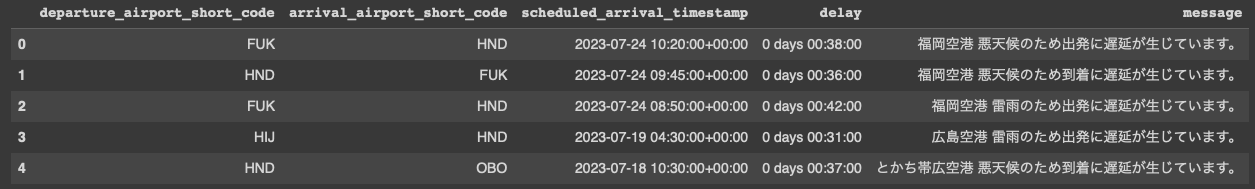
\includegraphics[width=12cm]{img/delay_data_sample.png}
        \caption{遅延データのサンプル}
        \label{fig:delay_data_sample}
    \end{center}
\end{figure}

\begin{figure}[htbp]
    \begin{center}
        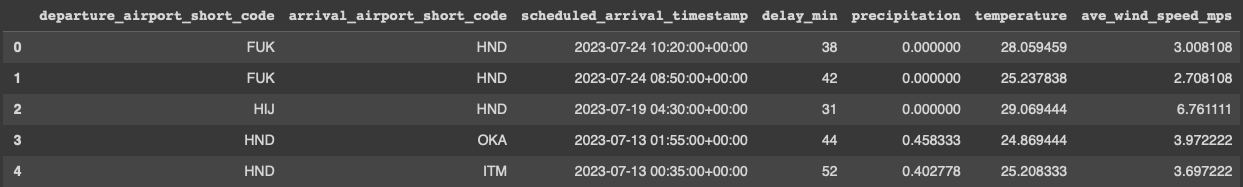
\includegraphics[width=12cm]{img/weather_data_sample.png}
        \caption{気象データのサンプル}
        \label{fig:weather_data_sample}
    \end{center}
\end{figure}

\section*{手法}

遅延データの備考には、発着空港のどちらの気象要因であるかが含まれている。そのため、どちらの空港に要因があるかによって、データを2つに分類した。

次に、遅延データと気象データを結びつける。到着予定時刻から、一定時間前までの気象データの平均値を、その遅延データに対応する気象データとした。遅延データは、到着空港への到着時刻のみであるため、出発時刻に関する情報がない。便名から出発時刻を調べることもできるが、今回は省略した。そのため、使用する気象データの範囲 (一定時間) は、次のように定めた。出発空港に要因があるデータ群に対しては、到着予定時刻から6時間前まで、到着空港に要因があるデータ群に対しては、到着予定時刻から3時間前までとした。

それぞれのデータ群を再び結合して、1つのテーブルにした。

気象データ (降水量、気温、平均風速) を説明変数、遅延データ (実際の到着時刻 - 予定されていた到着時刻) としたデータを重回帰分析し、どの気象要因が遅延時間に最も影響を与えているのかを調べる。

\begin{figure}[htbp]
    \begin{center}
        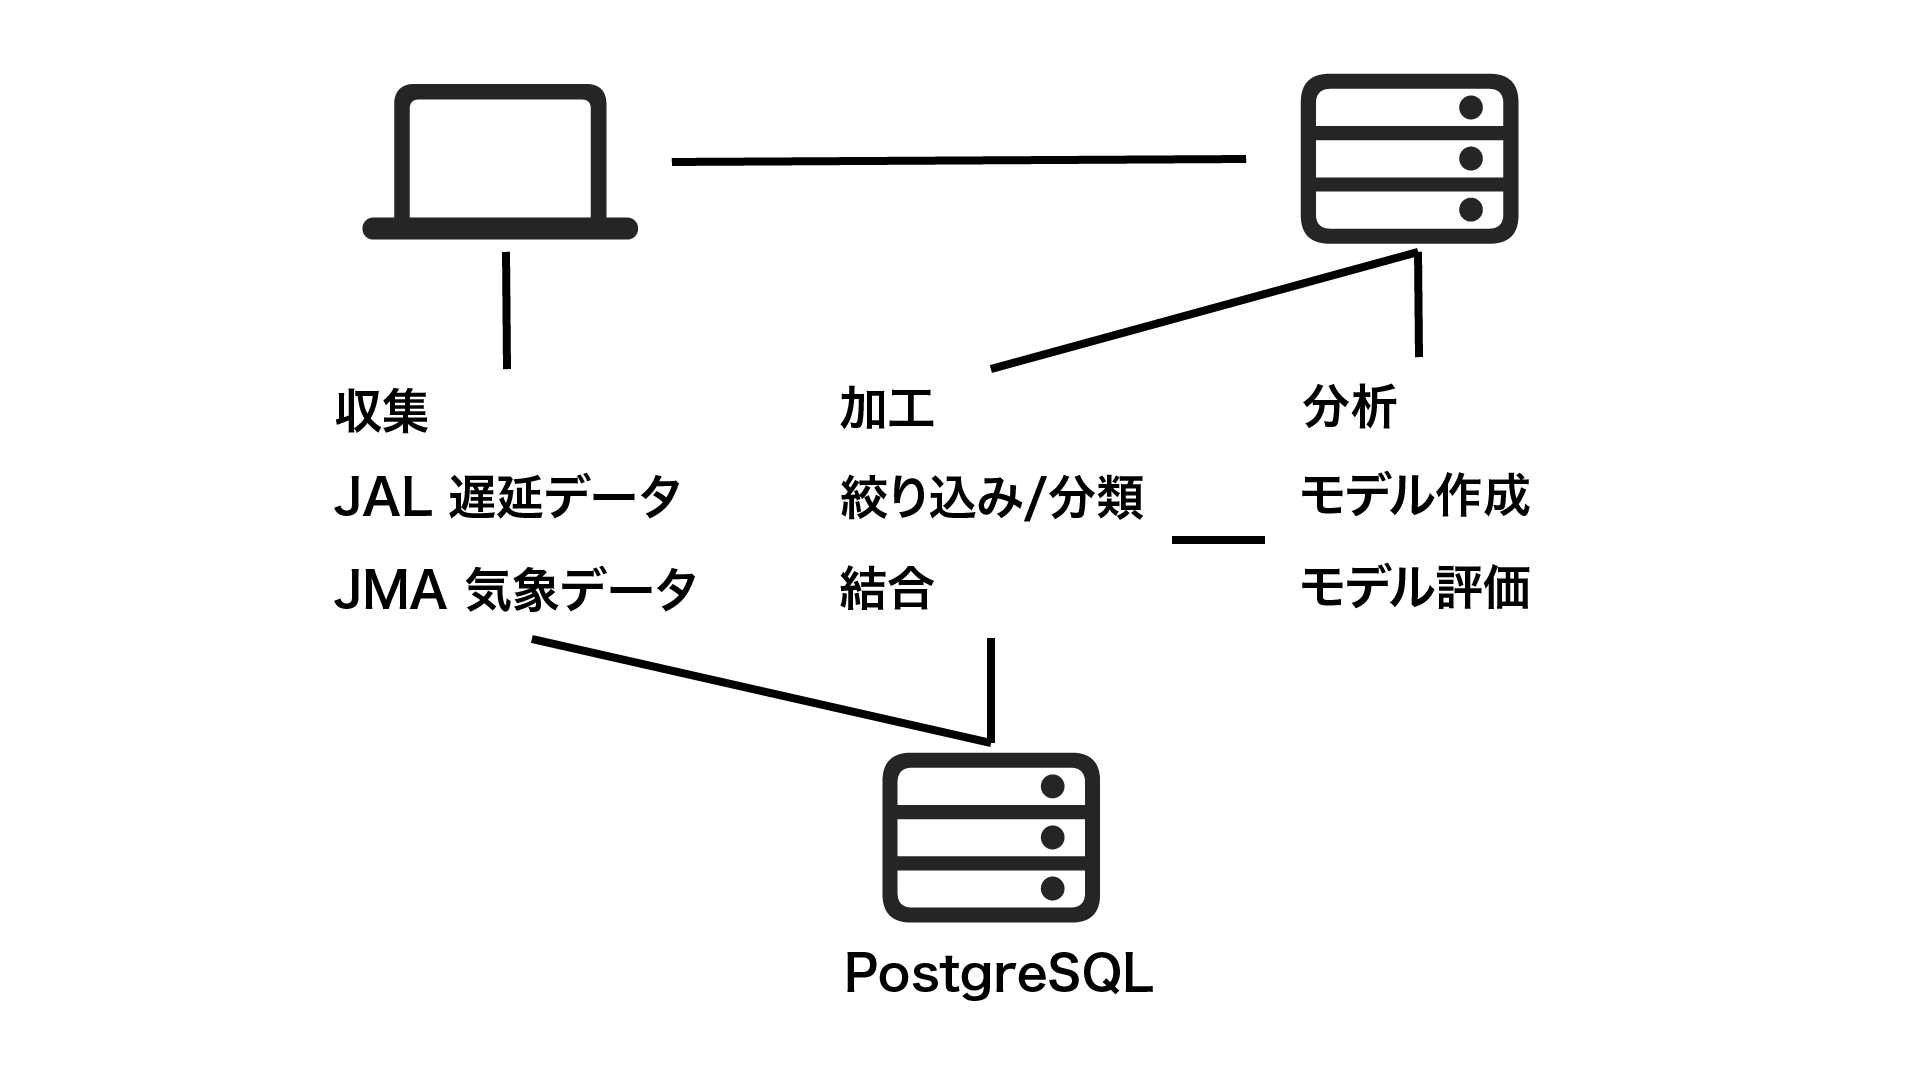
\includegraphics[width=12cm]{img/process.png}
        \caption{全体の流れ}
        \label{fig:process}
    \end{center}
\end{figure}

\section*{実装 (実験)}
動作環境として、AWSのAmazon EC2 G4dn インスタンス\cite{awsG4dn} (g4dn.xlarge) 上でJupyter Labを使用した。気象データ (降水量、気温、平均風速) を説明変数、遅延データ (実際の到着時刻 - 予定されていた到着時刻) を目的変数とした。これらをscikit-learnのLinearRegressionクラスを使用して、モデルを作成した。

\section*{結果}
テスト用のデータによる評価の結果、スコアは-0.73であった。また、訓練用のデータでも、0.06にとどまった。今回設定した説明変数同士に強い相関は見られなかった。決定係数は、降水量は-62.36、気温は-1.98、平均風速は、2.08という結果になった。

\section*{結論・考察}
決定係数のみを見ると、降水量は遅延時間の増加に負の影響を与え、その影響の大きさは最も大きく、風速のみが遅延時間の増加に正の影響を与えることがわかる。

しかし、モデルの評価の結果から、作成したモデルは、全く信頼性がないことがわかった。その要因として、分析の過程を振り返ったときに、次の3つの理由が考えられる。

1つ目は、遅延データの不足である。今回収集した、気象要因による遅延データは、27件にとどまってしまった。これは、遅延データを実験日から3週間前までのものしか得られなかったことが原因である。また、欠損値が含まれていたものを削除したため、さらに件数が減ってしまった。

2つ目は、遅延データと気象データを結びつける際に、一定時間前までの気象データの平均値を用いる際に、その幅の決定根拠が不明瞭である点である。到着時間しか得られなかったことで、正確性が落ちてしまったと考えられる。また、出発空港に原因があるデータ群に対して、実際の到着時刻の6時間前までの気象データの平均値を用いたが、出発空港を出発してからのデータは関係ないため、除くべきであったと考えられる。

3つ目は、2つ目の理由にも関連するが、そもそも飛行機の遅延時間は、離着陸の天候によって決まるものであって、その数時間前の天候の影響は直接受けない\cite{delayReason}。数時間前の天候と数時間後の天候の相関を調べる必要がありそうだ。

また、今回の調査では、遅延した時のデータのみを使用したが、遅延が発生しなかった時のデータも、遅延時間0として、気象データと結び付けた上で、モデルの学習に使うべきなのではないかと考えた。

今後はさらに時間をかけて、遅延データの質を上げ、遅延データと気象データの結び付けの方法を丁寧に議論して、再度分析したい。

\pagebreak

\bibliography{ref}

\pagebreak

\begin{appendix}

\section*{実験に用いたソースコード}
\lstinputlisting[language=Python]{code.py}

\end{appendix}

\end{document}
